\documentclass{article}
\usepackage[T1]{fontenc}
\usepackage{lmodern}
\usepackage{graphicx}
\usepackage{amsmath,amssymb}
\usepackage[a4paper,margin=2cm]{geometry}
\usepackage[absolute,overlay]{textpos}
\setlength{\TPHorizModule}{1mm}
\setlength{\TPVertModule}{1mm}
\usepackage[indonesian]{babel}
\usepackage{hyperref}
\setlength{\emergencystretch}{2em}
% unit: Halaman 106

\begin{document}

% === Halaman 106 (llm) ===

\section*{HILL CIPHER}
Cryptography $\cdot$ Poly-Alphabetic Cipher $\cdot$ Hill Cipher

\vspace{10mm}

\subsection*{HILL DECODER}

\textbf{CIPHERTEXT}

\vspace{151.47mm}

\begin{center}
\begin{tabular}{|c|c|}
\hline
17 & 17 \\ $\hline$
21 & 18 \\ $\hline$
2 & 2 \\ $\hline$
\end{tabular}
\end{center}

$\begin{aligned}
& \text{Try / Bruteforce all } 2\times2 \text{ matrix (values } 10 \le \text{ Latin Alphabet)}
& \text{I know the NON matrix numbers / values}
\end{aligned}$

$\begin{aligned}
& \text{Alphabet options:}
& \square \text{ ALPHABET (26 LET. A=0) ABCDEFGHIJKLMNOPQRSTUVWXYZ}
& \square \text{ ALPHABET (26 LET. A=1) ABCDEFGHIJKLMNOPQRSTUVWXYZ}
& \square \text{ ALPHABET (27 CHAR. A=0) ABCDEFGHIJKLMNOPQRSTUVWXYZ\_}
& \square \text{ ALPHABET (27 CHAR. A=1) \_ABCDEFGHIJKLMNOPQRSTUVWXYZ}
& \square \text{ CUSTOM ALPHANUMERIC ALPHABET}
\end{aligned}$

\vspace{5mm}

\subsection*{Summary}
\begin{itemize}
    \item Hill Decoder
    \item Hill Encoder
    \item Matrix Inversion
    \item What is the Hill cipher? (Definitions)
    \item How to encrypt using Hill cipher?
    \item How to decrypt Hill cipher?
    \item Why must the determinant of the Hill matrix be coprime with 26?
    \item How to decipher Hill without the key matrix?
    \item What are the variants of the Hill cipher?
    \item When was the Hill cipher invented?
\end{itemize}

\subsection*{Similar pages}
\begin{itemize}
    \item Affine Cipher
    \item Inverse of a Matrix
    \item Matrix Calculator
    \item Variant Beaufort Cipher
    \item Bellaso Cipher
\end{itemize}

% deskripsi: Screenshot antarmuka alat Hill Decoder dari situs dCode, menampilkan input teks cipher dan parameter matrix.
% bbox normalisasi: [0.3900, 0.4100, 0.6100, 0.9200]
\begin{textblock*}{46.20mm}(81.90mm,121.77mm)
\noindent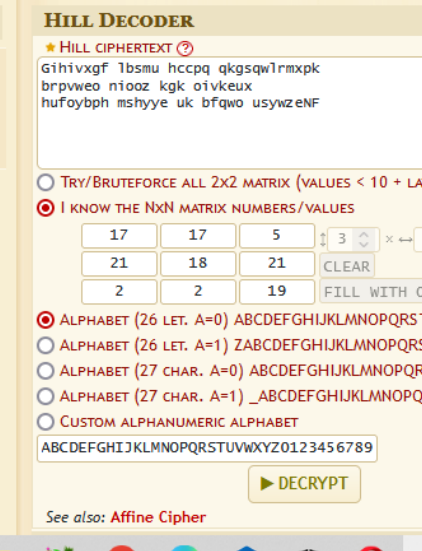
\includegraphics[width=46.20mm,height=151.47mm]{../../images/llm/page_106_img_01.png}%
\end{textblock*}

\end{document}
